\begin{figure}[ht] 
 	\centering 
 	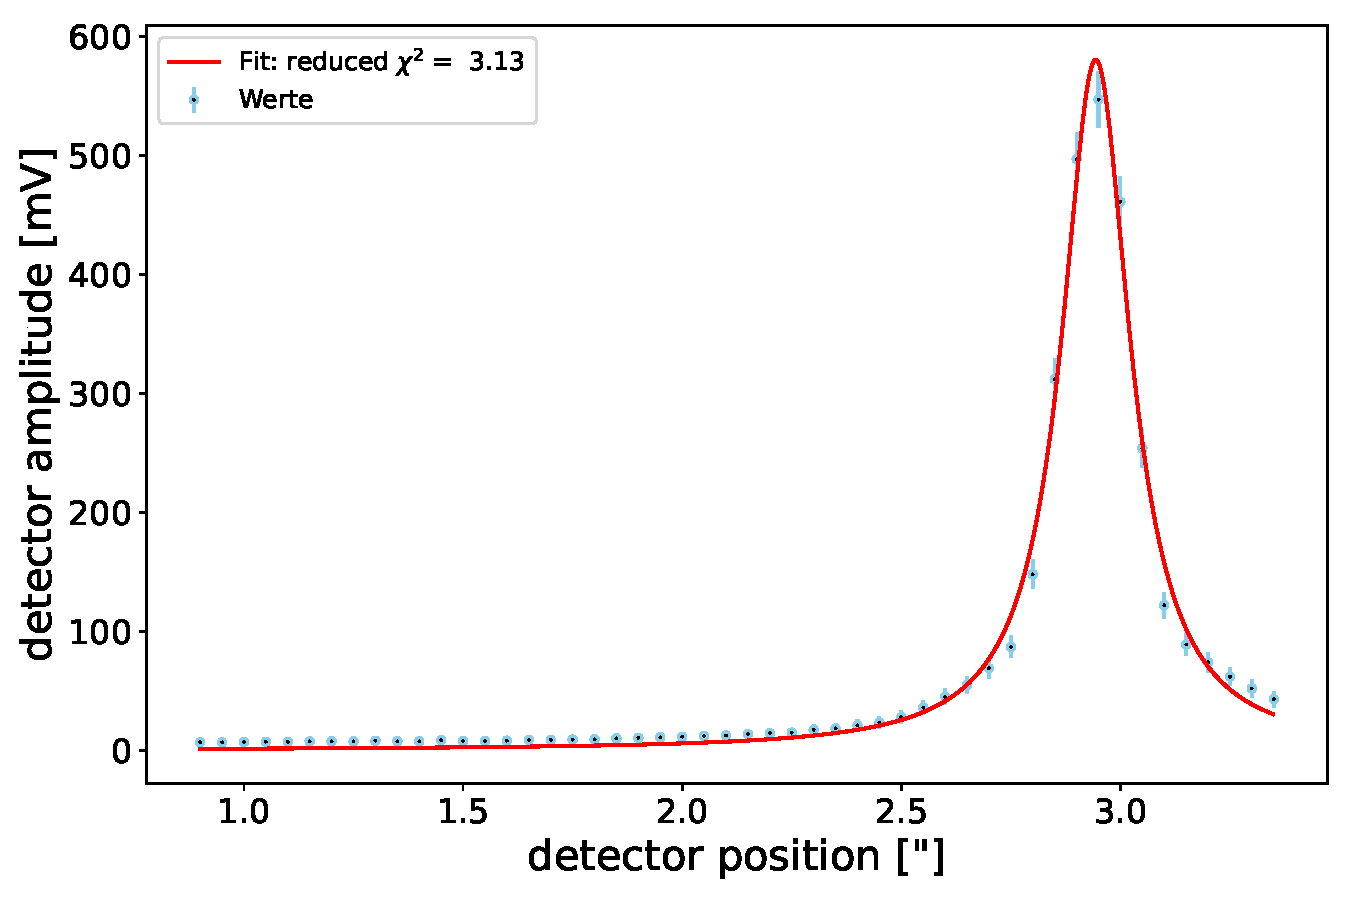
\includegraphics[width= 0.65 \textwidth]{Fits/Amps_B0A_Fit.pdf} 
	\caption{Amps_B0A, Fit} 
 	\label{fig:Amps_B0A, Fit} 
\end{figure}
 \\ 
\begin{table}[ht] 
\centering 
\caption{Amps_B0A, Fit Parameter Tabelle} 
\label{tab:my-table}
\begin{tabular}{|l|c|}
\hline
Parameter Name	&	Wert \\ \hline
amplitude	&	 174.313 \pm  5.585\\ \hline
center	&	 2.944 \pm  0.00409\\ \hline
sigma	&	 0.0966 \pm  0.0091\\ \hline
fraction	&	 0.998 \pm  0.0213\\ \hline
fwhm	&	 0.193 \pm  0.0182\\ \hline
height	&	 574.879 \pm  62.576\\ \hline
\end{tabular} 
\end{table}